\documentclass[a4paper,oneside,12pt]{book}

\usepackage[T1]{fontenc}
\usepackage[utf8]{inputenc}
\usepackage[english]{babel}
\usepackage[a4paper,top=2.54cm,bottom=2.54cm,left=2.54cm,right=2.54cm,headheight=16pt]{geometry}
\usepackage{amsmath}
\usepackage[pdftex]{graphicx}
\usepackage[colorlinks=true, allcolors=black]{hyperref}
\usepackage{hyperxmp}
\usepackage[format=plain, font=it]{caption}
\usepackage{sfmath}
\usepackage[parfill]{parskip}
\usepackage{setspace}
\usepackage{enumerate}
\usepackage{booktabs}
\usepackage{fancyhdr}
\usepackage{titlesec}
\usepackage[section,newfloat]{minted}
\usepackage{chngcntr}
\usepackage[backend=biber, style=numeric-comp, sorting=none]{biblatex}
\usepackage[autostyle=true]{csquotes}
\usepackage{xurl}
\usepackage{blindtext}

\addbibresource{references.bib}

\setlength{\marginparwidth}{2cm}
\pagestyle{plain}
\counterwithin{figure}{section}
\renewcommand{\familydefault}{\sfdefault}

\titleformat{\chapter}[hang]{\normalfont\huge\bfseries}{\thechapter}{1cm}{}{}
\title{A distributed deployment model for Encrypted Client Hello}
\author{Ted Johnson}

\begin{document}

\hypersetup{
	pdftitle=A distributed deployment model for Encrypted Client Hello,
	pdfauthor=Ted Johnson,
	pdfsubject=Master in Computer Science (MCS),
	pdfinfo={pdfsupervisor=Dr Stephen Farrell},
	linkcolor=black,
	citecolor=blue,
	filecolor=blue,
	urlcolor=blue
}
\urlstyle{same}
\definecolor{bg}{rgb}{0.95,0.95,0.95}
\setminted{
	bgcolor=bg,
	fontsize=\footnotesize,
	linenos=true,
	numbersep=5pt,
	tabsize=4
}

\frontmatter
\hypersetup{pageanchor=false}

\begin{titlepage}

\center


\includegraphics{images/trinity_college_dublin.png}\\[1cm]
\Large \href{https://www.tcd.ie/scss/}{School of Computer Science and Statistics}\\[1.5cm]
\makeatletter{\huge \bfseries A distributed deployment model for Encrypted Client Hello}\\[1.5cm]
Ted Johnson\\[2cm]
Supervisor: Dr Stephen Farrell\\[2cm]
{\large April 2024}\\[2cm]

\vfill

A dissertation submitted in partial fulfilment\\
of the requirements for the degree of\\
Master in Computer Science (MCS)

\vfill

\end{titlepage}

\hypersetup{pageanchor=true}

\section*{\Huge{Declaration}}

\vspace{1cm}
I hereby declare that this dissertation is entirely my own work and that it has not been submitted as an exercise for a degree at this or any other university.

\vspace{1cm}
I have read and I understand the plagiarism provisions in the General Regulations of the University Calendar for the current year, found at \url{http://www.tcd.ie/calendar}.

\vspace{1cm}
I have completed the Online Tutorial on avoiding plagiarism `Ready Steady Write', located at \url{http://tcd-ie.libguides.com/plagiarism/ready-steady-write}.

\vspace{1cm}
I consent to the examiner retaining a copy of the thesis beyond the examining period, should they so wish (EU GDPR May 2018).

\vspace{3cm}
Signed:~\rule{5cm}{0.3pt}\hfill Date:~\rule{5cm}{0.3pt}

\chapter*{}
\thispagestyle{empty}
\addcontentsline{toc}{chapter}{Abstract}

\vspace*{0mm}
\begin{center}
\setlength{\unitlength}{1mm}

\begin{spacing}{2}
\textbf{\Large A distributed deployment model \\ for Encrypted Client Hello} \\[10mm]
\end{spacing}

\begin{spacing}{1.5}
Ted Johnson, Master in Computer Science \\
University of Dublin, Trinity College, 2024 \\[10mm]
\end{spacing}

Supervisor: Dr Stephen Farrell \\
\end{center}
\vspace{5mm}

\begin{spacing}{1} \noindent
Encrypted Client Hello (ECH) is a proposed extension to the Transport Layer Security (TLS) protocol that encrypts information currently leaked during connection, which is now beginning to see implementation and adoption on the Internet. However, typical deployment strategies encourage placing many TLS servers behind a single ECH-service provider to form an anonymity set, which introduces significant network centralisation and limits the types of environments the extension can be operated in.

This report presents a method for distributing the deployment of ECH amongst a loose network of co-operating TLS servers, such that each server functions as an ECH-service provider for all others. This allows for ECH-enabled clients to access services through any co-operating TLS server, greatly strengthening service availability and network flexibility. The effectiveness of this solution is evaluated based on its privacy and security implications, impact to overall network performance and ability to fairly allocate load between participating servers over time.
\end{spacing}

\newpage
\onehalfspacing
\raggedright
\section*{\Huge{Acknowledgements}}

\blindtext
% \begin{spacing}{1.5}}
% {\end{spacing} \par \vspace{20mm}
% \raggedleft Ted Johnson \\[10mm]
% \raggedright {{\slshape
% \renewcommand{\arraystretch}{1.0}
% \begin{tabular}{l}
% University of Dublin, Trinity College \\
% April 2024
% \end{tabular}}} \newpage}


\tableofcontents
\listoffigures
\listoflistings
\newpage

\mainmatter
\chapter{Introduction}\label{Introduction}

Encrypted Client Hello (ECH) is a proposed extension to the Transport Layer Security protocol version 1.3 (TLS 1.3) which has begun to see implementation and adoption on the Internet~\cite{tsiatsikas2022measuring, CF-ECH}. ECH seeks to allow encryption of the ClientHello message, which can contain potentially sensitive information such as the Service Name Indication (SNI) and Application-Layer Protocol Negotiation (ALPN) extensions. This is partially achieved through serving many private domains behind a common provider to form an anonymity set that conceals the true domain requested by the client.

Due to this, ECH introduces significant centralisation to the Internet. This paper presents a practical model for the distributed deployment of ECH amongst several co-operating TLS servers, where each server operates both as the origin server of its own domains as well as an ECH provider for other participating servers. The model addresses a number of implementation challenges, predominately related to ensuring the security of the protocol is not compromised and minimising the performance impact to the connection while strengthening service availability.

Included in this paper is a review of the background technology and concepts relevant to the discussion of the deployment model. This is followed by a study of the model's design and the complications which influenced it. We then see how this design can be implemented within a practical scenario and discuss some of its deployment considerations. In the subsequent chapter, an analysis and criticism of both the results taken from this implementation and the design as a whole is used to assess the quality of the solution. Finally, I conclude the report with a summary of the work completed and delineate where future contributions could best benefit the further development of the deployment model.









\section{Motivation}

Mark Nottingham has previously cautioned against the introduction of centralisation through Internet standards~\cite{rfc9518}. Of particular relevance to ECH is his highlight of the adverse effect centralisation can have on infrastructure resilience and service availability through reliance on a single entity. This is especially detrimental to ECH where the effectiveness of its anonymity set grows with the number of private domains served by a single provider. Nottingham also writes on susceptibility of centralisation to stifle innovation and induce an unhealthy monoculture which may result in less overall technological progress and robustness of the ECH protocol.

Additionally, allowing entirely independent servers to co-operate from across the Internet to provide ECH support for each other enables several distinct organisations to work together to offer improved privacy for their users without the requirement for co-located servers nor the dependence of any on the availability on another. Consider here global networks of whistleblower services, investigative journalists and human rights non-profit organisations who share an interest in protecting the confidentiality of their members and users from persecution and retaliation.

For these reasons, the development of a model for the distributed deployment of ECH across several co-operating providers is a key step towards its application in <perilous> scenarios and broad adoption throughout the Internet.









\section{Project Objectives}

The objectives of this research project can be summarised with the following question: ``How can Encrypted Client Hello be deployed fairly amongst co-operating Transport Layer Security servers to reduce network centralisation without compromising the security of the protocol?'' This task is composed of the following objectives:

\begin{description}
	\item[1. Identify principal challenges and appropriate solutions.] Before development can begin proper, we must first understand the environment the system would operate in and explore the technical and logistical issues it might face to determine the dominant criteria for design. We accomplish this through research and experimentation of the functioning of the protocol and its surrounding technologies.
	\item[2. Design, evalute and contrast deployment models.] An iterative development process is used to produce a series of incrementally improved skeletal prototypes, with the goal to rapidly design and test for functionality guided by the design criteria and results of previous work as heuristics.
	\item[3. Analyse model implementatons through simulation.] Promising design solutions are fleshed out into full implementations within deterministic, reproducible and quantifiable simulated environments, where security and performance implications can be easily isolated and compared. It is expected that unforeseeable practical challenges and considerations are to be unveiled during this work.
	\item[4. Conclude findings.] <Learnings from comparisons> <As part of this, a prototype script is to be compiled from the implementation snippets>
\end{description}

In preparation for undertaking this project, I had produced the Gantt chart included in Fig.~\ref{gantt_chart_figure} to help gauge my progress during the four months of work. While I found more emphasis has been placed on implementation, the overall task structure of the timeline has been followed reasonable well.

\begin{figure}[ht]
\centerline{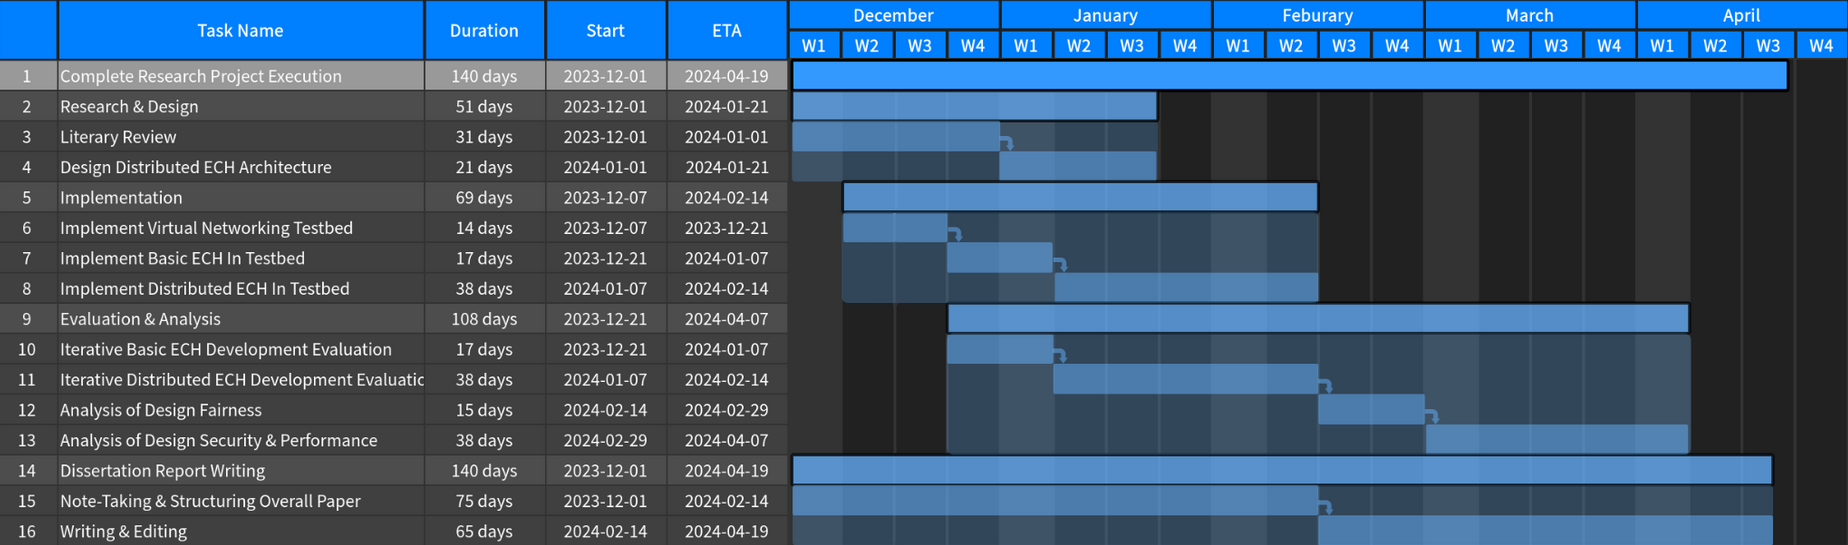
\includegraphics[width=160mm]{images/gantt.png}}
\caption[Project timeline]{Predicted timeline of project as of the 7\textsuperscript{th} of December, 2023}
\label{gantt_chart_figure}
\end{figure}









\section{Research Contributions}

This work provides evidence for the viability of the distributed deployment of ECH between co-operative TLS servers. It supports its argument that the deployment model presented does not compromise the security of the protocol and minimises impact to network performance though analysis of the data produced by implementations within simulated networking environments. Additionally, an evaluation of several traffic masking and normalisation techniques is given to serve as the bases for further work on disrupting traffic correlation attacks applicable to ECH and elsewhere. Finally, the delivered project may also contribute academic value as a deterministic, reproducible tutorial on the deployment and operation of ECH using commonplace software and tooling.

\chapter{Background}\label{Background}

This chapter offers an overview of the technology and concepts needed to understand the context and relevance of the work within the broader world. The review is conducted predominately through a networking, security and privacy perspective to best highlight the aspects pertinent to the distributed deployment of ECH. This chapter also represents the bulk of the effort put into investigating and studying the functioning of ECH while identifying and experimenting with different deployment models.

The contents of this chapter include a high level description of the Transport Layer Security protocol and the Domain Name System with a more detailed look at the components that enable ECH functionality. This is followed by an inspection of ECH itself, its security properties and the mechanisms which allow for distributed deployment. Finally, we survey how a variety of traffic analysis techniques that can be used to infer sensitive information from patterns in network activity, as well as the countermeasures which exist to mask these patterns.








\section{Transport Layer Security}

Transport Layer Security (TLS) is a cryptographic protocol proposed by the Internet Engineering Task Force (IETF) which enables secure communication over public networks. Applications and services can establish an encrypted communication channel to transmit private information such that confidentiality, integrity and authenticity of the data can be ensured. TLS is commonly used to protect Internet traffic, having seen widespread adoption and several revisions since its original inception in 1999, superseding the Secure Sockets Layer (SSL) specifications previously defined by Netscape Communications~\cite{chan2018monitoring, LE-HTTPS, rfc2246}.

TLS is designed to operate on top of a reliable transmission protocol between a client and server, typically the Transmission Control Protocol (TCP) when used over the Internet. In order to prevent eavesdropping, tampering and message forgery, TLS includes a number of security features based on a number of cryptographic mechanisms:

\begin{description}
\item[Confidentiality:] All service and application data exchanged between the client and server is encrypted as to make it indecipherable to any intermediate party which might be intercepting their communication. For example, consider the importance of protecting passwords, banking information and patient health records.
\item[Data integrity:] In a similar manner, cryptographic properties are used to guarantee transferred data cannot be modified during transmission. This is critical for safeguarding against input manipulation in consequential situations, such as while specifying fields for a financial transaction.
\item[Authentication:] TLS provides the ability for both peers to verify the identity of the other, ensuring privileged communication is only performed with the intended recipient. Such a condition is fundamental for establishing trust and confidence in any sensitive environment.
\end{description}

TLS 1.3 is the latest defined standard for the protocol, having been published in August 2018 and contributing to the deprecation of TLS 1.0 and TLS 1.1 in March 2021~\cite{rfc8446, rfc8996}. Lee, Kim, and Kwon have measured a comparatively rapid adoption rate, reporting support by 48\% of Alexa top 1M sites by 2021, which is attributed largely to the growth of cloud hosting providers such as Cloudflare~\cite{holz2019era, lee2021tls}. The version introduces many major changes over TLS 1.2, including the addition of a zero round trip time resumption (0-RTT) mode, further encryption and optimisation of the handshake and removal of outdated cryptographic algorithms and security mechanism with all key exchanges now providing forward secrecy. A change of particular relevance to ECH is the encryption of the digital certificate received by the client to authenticate the server.

\subsection{Digital Certificates}

TLS uses X.509 digital certificates to make assertions on the identity of entities within the network using a chain of trust model, and are intrinsic to the authentication within the public key infrastructure used to initiate a secure TLS key exchange~\cite{rfc4158}. Without this assertion in place, a malicious party may insert itself into the middle of any TLS connection to perform a man-in-the-middle attack by replacing any public key with their own outside the knowledge of either peers. This invalidates the security of the key exchange and thus compromises any security offered by TLS. Therefore, to have any confidence in a secure connection, we must be able to trust the authenticity of received public keys by associating them with a trustworthy digital certificate.

It is not feasible to have a trusted party for every entity install a certificate for every other entity, as this becomes impractical within larger networks in which certificates may be created and replaced. Instead, this trustworthiness is established through the associativity, where cryptographic signatures provide a mechanism for one certificate to attest to the validity of another as depicted in Fig.~\ref{tls_chain_figure}. A Certificate Authority (CA) may issue new certificates using their private key to produce a signature that can be authenticated using the public key present in their own certificate. Furthermore, the certificate of the CA was issued by its parent CA and contains a signature which itself can be authenticated in a similar manner. In this way, certificates are organised into a hierarchical chain of trust, where the trustworthiness of a certificate is asserted by the trustworthiness of its issuer. This chain of trust continues until a root certificate issued by a root CA using a self-signed signature is encountered at the base of the hierarchy, which is implicitly trusted by all entities.

\begin{figure}[ht]
\centerline{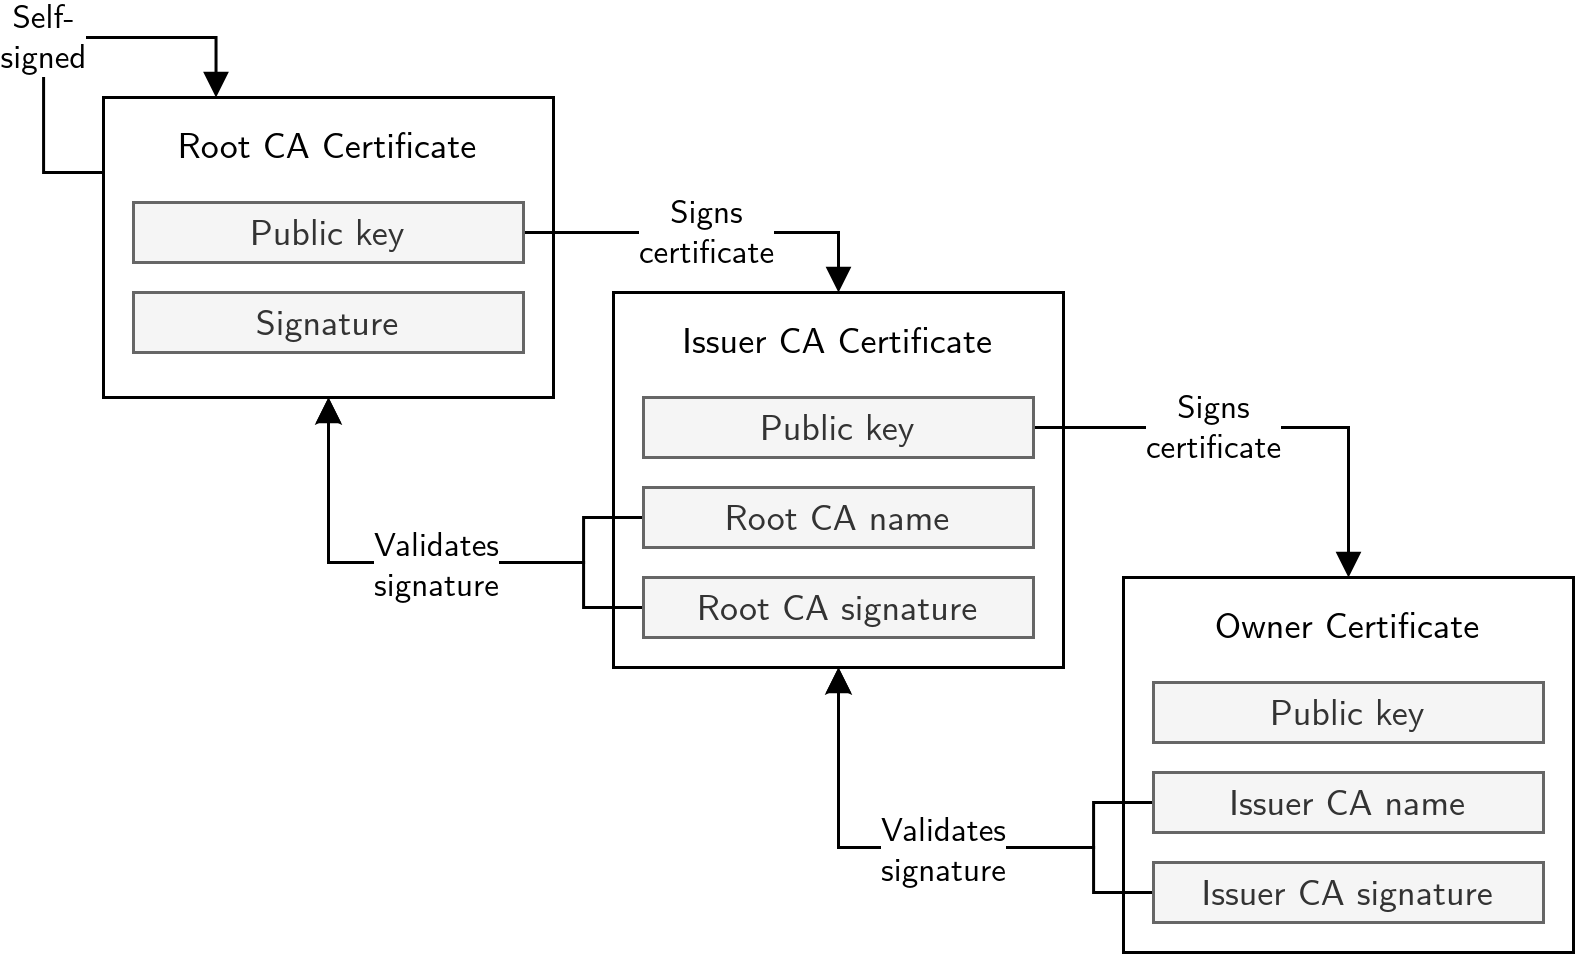
\includegraphics[width=160mm]{images/tls-chain.png}}
\caption[TLS certificate chain of trust]{A chain of trust established between the unknown owner certificate and the implicitly trusted root CA certificate in order to authenticate the identity of the owner against its associated public key.}
\label{tls_chain_figure}
\end{figure}

An organisation or individual must request new certificates from a CA using a Certificate Signing Request (CSR). The CA is then responsible for verifying the identity of the organisation or individual before issuing the certificate. To ensure the validity of certificates are consistent over time, X.509 certificates expire after a set period and must be renewed. Today, this renewal procedure has been widely automated using the Automatic Certificate Management Environment (ACME) protocol, which allows for web servers to complete challenges set by the CA to prove ownership of their domain name and public key without human involvement~\cite{rfc8555}. This has enabled a much shorter certificate rotation period, and it is common to see certificates set to expire within three months.

Through this process, an entity is only required to trust a few well-established root certificates to be capable of validating the authenticity of many certificates and their public keys. These root certificates are generally installed by an inherently trusted party such as the device manufacturer or operating system, but new certificates may be installed by the user.

Typically on the Internet, it is only necessary for the identity of the server be authenticated by the client, while the client remains unauthenticated to the server in the TLS context. In either case, certificates may be exchanged between the server and client during the TLS handshake.

\subsection{TLS 1.3 Handshake}

The TLS handshake is the series of messages exchanged between the client and server to establish the connection. It specifies the steps required to negotiate connection parameters, authenticate peer identities and yield a shared secret. TLS 1.3 was designed to improve the security and performance of the handshake over TLS 1.2 while reducing its overall complexity. Highlighted in these changes is the integration of parameter negotiation into the first client message, enabling encryption of much more of the handshake as well as allowing application data to be sent by the client after only one round trip.

\begin{figure}[ht]
\centerline{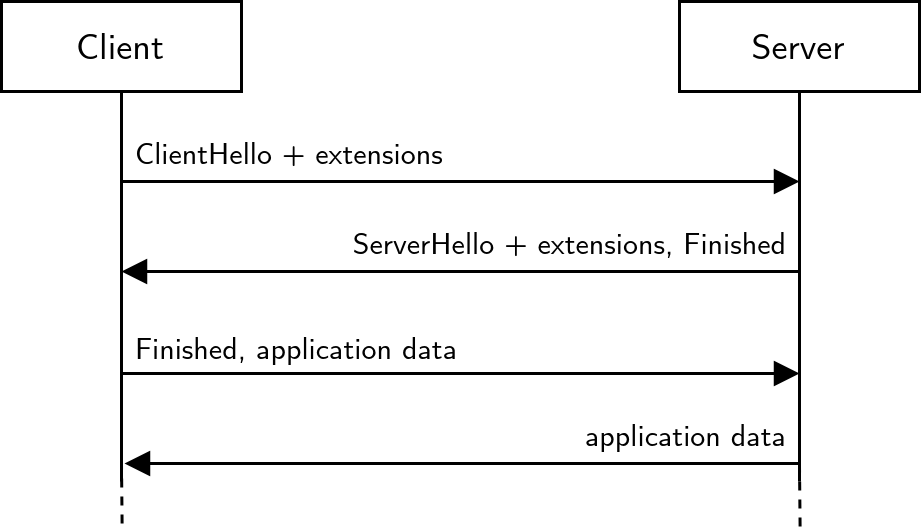
\includegraphics[width=120mm]{images/tls-handshake.png}}
\caption[Basic TLS 1.3 handshake]{Sequence diagram between a client and server describing a basic TLS 1.3 handshake with only server authentication.}
\label{tls_handshake_figure}
\end{figure}

Once a reliable transmission channel has been created between the client and server, a TLS 1.3 handshake can be performed as seen in Fig.~\ref{tls_handshake_figure}. The core functionality of the handshake can be achieved in as few as four message types:

\begin{description}
	\item[ClientHello:] The client initiates the handshake by sending a ClientHello message without any encryption, containing information such as the supported TLS version number, along with a list of available cipher suites and their parameters for the server to choose from. Included in this is also an optimistic key share using the client's preferred cipher suite key exchange method, namely Diffie-Hellman (DH) or Elliptic Curve Diffie-Hellman (ECDH). Both of these generate ephemeral keys for each session, ensuring forward secrecy is preserved in the event the server's private key is compromised. Finally, the ClientHello message also contains a random value generated by the client used to prevent replay attacks.
	\item[ServerHello:] If the server supports the client's preferred cipher suite, it is able to continue the key exchange immediately in the ServerHello message. Otherwise, the server must send a HelloRetryRequest to restart the key share with a different key exchange method which requires an additional round trip. The ServerHello message is sent without encryption and informs the client of what cipher suite and parameters were selected, as well as includes its own random value generated by the server. As the server has now completed its side of the key exchange, all subsequent communication is now encrypted using the selected symmetric encryption algorithm, such as AES-GCM or ChaCha20-Poly1305.
	\item[Certificate:] The server then sends the client its certificate and proof of private key possession by signing a cryptographic hash of the transcript of the handshake so far. It may also choose to request authentication from the client using a CertificateRequest message, which requires the client to respond with its own Certificate message and proof of private key possession.
	\item[Finished:] Finally, the server concludes its side of the handshake by initiating an exchange of Finished messages with the client. This message consists of a Message Authentication Code (MAC) over the cryptographic hash of the transcript of the entire handshake. In this way, the client can confirm success of the key exchange and integrity of the transaction. Once the client has received the ServerHello with the completed key exchange as well as decrypted and validated the Certificate and Finished message, it produces its own Finished message for the server to perform the same checks. Finally, with both peers in agreement on the security of the connection, application data can begin to be securely exchanged.
\end{description}

There are many more complexities to this handshake which are not particularly relevant here that have been omitted from this overview for the sake of brevity. However, one important topic to mention is the inclusion of extensions.

\subsection{Extensions}

Within both the TLS 1.2 and TLS 1.3 handshakes, the ClientHello and ServerHello messages may be extended with additional functionality, which allows the protocol to fulfil a wider range of use cases and accommodate evolving requirements. The usage of extensions has been significantly expanded in TLS 1.3 and now includes the ability for previously unencrypted ServerHello extensions to be placed within the new EncryptedExtensions message sent after ServerHello. Furthermore, a number of new extensions have been defined and several extensions are mandatory to include in the TLS 1.3 handshake. Indeed, the Key Share extension is the provided mechanism for performing key exchanges and the Supported Versions extension is used to signify which versions of TLS is supported.

Nevertheless, the ClientHello message is not encrypted and all of its extensions are sent in the clear. Some of the ClientHello extensions include potentially sensitive information such as the Server Name Indication (SNI) and Application Layer Protocol Negotiation (ALPN) list. It is this privacy weakness that the purposed ECH extension is attempting to remedy.









\section{The Domain Name System}

The Domain Name System (DNS) was designed by Mockapetris in 1984 as a replacement for the manually maintained and shared HOSTS.TXT file used in Internet Protocol (IP) networks to map hostnames to IP addresses, which was becoming increasingly impractical as networks grew in size and complexity~\cite{rfc1034, rfc1035}. Instead, DNS offers a naming system that associates hierarchical alphanumeric identifiers, referred to as domain names, with various resource records, like IP addresses. In this context, a zone is defined as the set containing a domain and all of its subdomains.

Citing significant scalability concerns due to the expected size of the service and the frequency of resource record updates, Mockapetris listed the distributed storage and management of domain name entries with local caching as a design goal for DNS. To address this, the naming system information is distributed as zones amongst many name servers such that each name server is capable of either directly operating on the requested domain name resource records or referring to another name server which is hierarchically closer to the requested domain name. The name server which manages a zone is considered the authoritative name server for the zone. With this, DNS can be used to translate from the more flexible and easily remembered domain names into the associated IP addresses and other resources required to access network applications and services.

\subsection{Name Resolution Process}

A client attempting to resolve a domain name may invoke requests across several name servers. Typically, the client operates as a stub resolver which delegates the task to a known recursive resolver, such as through their network router or Internet service provider (ISP). This is generally done to allow for the caching of DNS query results for use by a whole network or organisation. This situation can be seen in Fig.~\ref{dns_resolve_figure}, where the client has requested the recursive resolver to retrieve resource records for `www.example.com'. To execute the DNS query, the recursive resolver needs to locate the authoritative name server for the requested domain name. Without prior knowledge or cached results, the resolver first queries one of the well-known root name servers to begin navigation of the name hierarchy. In accordance with the distributed nature of DNS, the root name server does not contain the resource records for the requested domain name, but instead directs the resolver to the top-level domain (TLD) name server for `.com'. The resolver reiterates its query to the TLD name server and is again pointed further down the hierarchy, this time to the authoritative name server for `example.com'. Finally, the resolver queries this name server and retrieves the request resource records, which are then returns to the client. All of these results are cached by the recursive resolver for a set amounts of time as specified by the Time To Live (TTL) contained within all responses to help reduce overall load on the system, especially root name servers.

\begin{figure}[ht]
\centerline{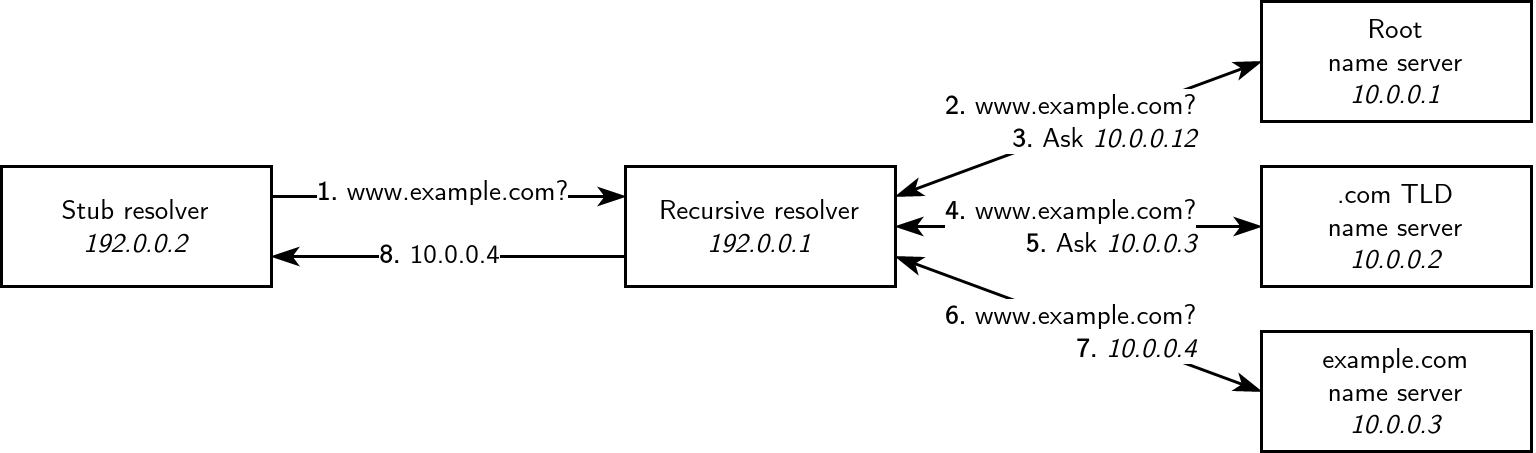
\includegraphics[width=160mm]{images/dns-resolve.png}}
\caption[Example DNS name resolution process]{A stub resolver requests a recursive resolver to retrieve resource records for `www.example.com'. Without previously cached query responses, the recursive resolver must navigate the domain name hierarchy starting at a known root name server.}
\label{dns_resolve_figure}
\end{figure}

\subsection{DNS over HTTPS}

Notably, Mockapetris makes no mention of security nor privacy in the original DNS specification and such concerns have only begun to be addressed in recent years, as summarised by Bortzmeyer in 2015~\cite{rfc7626}. This has largely been due the naming system information being perceived as public knowledge and not requiring security mechanisms. As such, DNS query and response communication have historically been sent unencrypted using the User Datagram Protocol (UDP). It has not been until the last decade with the revelations of widespread global surveillance that issues such as these have started to see much more attention. In 2013, Cooper et al. wrote extensively on the formulation of privacy threats and mitigations for consideration during the design of Internet protocols, and lists surveillance as being a prevalent privacy threat~\cite{rfc6973}. Following this, Farrell and Tschofenig emphasised the danger of exposing protocol content and metadata to large scale surveillance operations and recommends mitigation through security-conscience protocol design~\cite{rfc7258}.

In an effort to apply these learnings, both DNS over TLS (DoT) and DNS over HTTPS (DoH) were conceived as methods for performing privacy-preserving DNS queries~\cite{rfc7858, rfc8484}. Both protocols add confidentiality and data integrity to DNS by encapsulating queries and responses inside secure TLS channels. The most notable difference between the standards is the port number used, as DoT traffic goes to the non-standard port 853 while DoH is served through the standard HTTPS port 443. This difference has lead to some adoption problems with DoT when compared to DoH, as it is not unusual for network firewalls to prohibit traffic to non-standard ports. This also has the effect of making DoT usage being quite conspicuous, while DoH disguises itself amongst other HTTPS traffic. Garc{\'\i}a et el. list these as factors when measuring a wider adoption of DoH in 2021~\cite{garcia2021large}.

\subsection{The HTTPS Resource Record}

Today, a number of DNS resource record types exist to fulfil more complex requirements and introduce advanced capabilities. The HTTPS resource record and the more general Service Binding (SVCB) resource record have recently been standardised to allow for specification of additional parameters related to service endpoint discovery and connection establishment~\cite{rfc9460}. This enables more information to be provided to the client needed to access a service while helping to avoid unnecessary round trips and DNS queries. This information set can include items such as the preferable IP address, port number and ALPN list used to connect to a service endpoint which must otherwise be retrieved separately through potentially suboptimal channels.

While ostensibly useful for reducing overall connection latency, the ability for these new resource records to associate parameters with service endpoints facilitates much more flexibility within DNS. In particular, the ECH extension delegates public key and metadata dissemination to this mechanism though the specification of an appropriate `ech` parameter for each service endpoint.








\section{Encrypted Client Hello}

Encrypted Client Hello (ECH) is a proposed extension to TLS 1.3 which has begun to see implementation and adoption on the Internet~\cite{ietf-tls-esni-18, tsiatsikas2022measuring, CF-ECH}. ECH seeks to allow encryption of the ClientHello message, which can contain potentially sensitive information such as the SNI and ALPN extensions. Exposure of the target domain name of the client's request through the SNI was previously considered acceptable due this information being revealed through other channels, but these leaks are becoming less exploitable: Cloud hosting providers, content delivery networks (CDNs) and reverse proxies have diluted the mapping from IP addresses to domain names, the use of encrypted DNS such as DoH is now concealing client DNS queries and the TCP 1.3 handshake encrypts the server certificate. As we have seen in the previous sections, the TLS and DNS ecosystems have adapted to new security and privacy expectations in recent years and are now equipped to support ECH.

The functionality of ECH is based on clients using the public key of an ECH-service provider to send an encrypted TLS 1.3 ClientHello message, which the provider decrypts and uses to proxy the TLS 1.3 connection to the true origin server. This provider may be common to many origin servers hosting many private domains that together form an anonymity set. The provider must first generate an ECH encryption key pair and some associated metadata. This public key and metadata, referred to as an ECH configuration or ECHConfig, may then be shared out-of-band with ECH-enabled clients though a secure context like DoH using the `ech' parameter in HTTPS resource records. A client may then use this public key and metadata to construct a ClientHello message, named the ClientHelloOuter, holding unremarkable values for the provider alongside the ECH extension containing an encrypted ClientHello, named the ClientHelloInner, itself holding the real values for a private domain. To establish a TLS connection to the origin server of this domain, the client initiates a TLS connection using the ClientHelloOuter with the provider, which decrypts the ClientHelloInner and relays the connection to the origin server, which itself completes the TLS handshake with the client through the provider. Importantly, the provider is incapable of eavesdropping on this secure channel, as the TLS connection is authenticated and end-to-end encrypted between the client and origin server.

\subsection{Hybrid Public Key Encryption}

ECH uses the Hybrid Public Key Encryption (HPKE) specification for performing public key encryption~\cite{rfc9180}. HPKE defines a standard scheme for combining the benefits of asymmetric and symmetric cryptographic algorithms such that the performance of symmetric cryptography can be gained where only the public key of the receiver is known. This is achieved through using the public key of the receiver to generate a symmetric encryption key as well as an encapsulated shared secret. This encapsulated shared secret can be sent to the receiver which can generate the symmetric encryption key using its private key. Any ciphertext produced by the sender with the symmetric encryption key can now be decrypted by the receiver.

HPKE defines several possible configurations of cryptographic parameters, namely selecting the key encapsulation mechanism (KEM), key derivation function (KDF) and Authenticated Encryption with Associated Data (AEAD) symmetric encryption algorithm. In ECH, these are defined to be elliptic-curve Diffie–Hellman (ECDH) using Curve25519, hashed message authentication code (HMAC) KDF (HKDF) and Advanced Encryption Standard (AES) in Galois/Counter Mode with 128-bit key sizes (AES-128-GCM), respectively. The KEM and KDF are able to produce the AES key and encapsulated shared secret from the contents of an ECHConfig generated by the ECH-service provider. AES encrypts the ClientHelloInner and ensures the ClientHelloOuter can not be tampered using its additional authenticated data (AAD) mechanism. Once the ClientHelloOuter containing the ECH extension is received, the provider can derive the same AEAD key from the encapsulated shared secret using the KDF with its private key and then decrypt the ClientHelloInner. Bhargavan, Cheval, and Wood have been able to verify the security of HPKE in the context of ECH through extensive formal analysis of the privacy properties of the TLS 1.3 handshake~\cite{bhargavan2022symbolic}.

\subsection{Split Mode Deployment}

The ECH protocol is designed to operate within two types of network topologies, referred to as Shared Mode and Split Mode. When in Shared Mode, the ECH-service provider and private domain origin server are the same network entity. The TLS 1.3 connection initiated by ECH-enabled clients with the provider is also completed by the provider, which can then serve the client the covertly requested domain name service. Split Mode relaxes this restriction to allow the physical separation of the provider and origin server. An example execution of ECH in Split Mode is visualised in Fig.~\ref{ech_split_mode_figure}, where we see the client again initiates a TLS 1.3 connection with the provider, but this connection is forwarded to the appropriate origin server which completes the connection. In either case, the true ClientHello message is still masked from network observers and the anonymity set consists of all possible private domains served via the provider using ECH Shared Mode or Split Mode.

\begin{figure}[ht]
\centerline{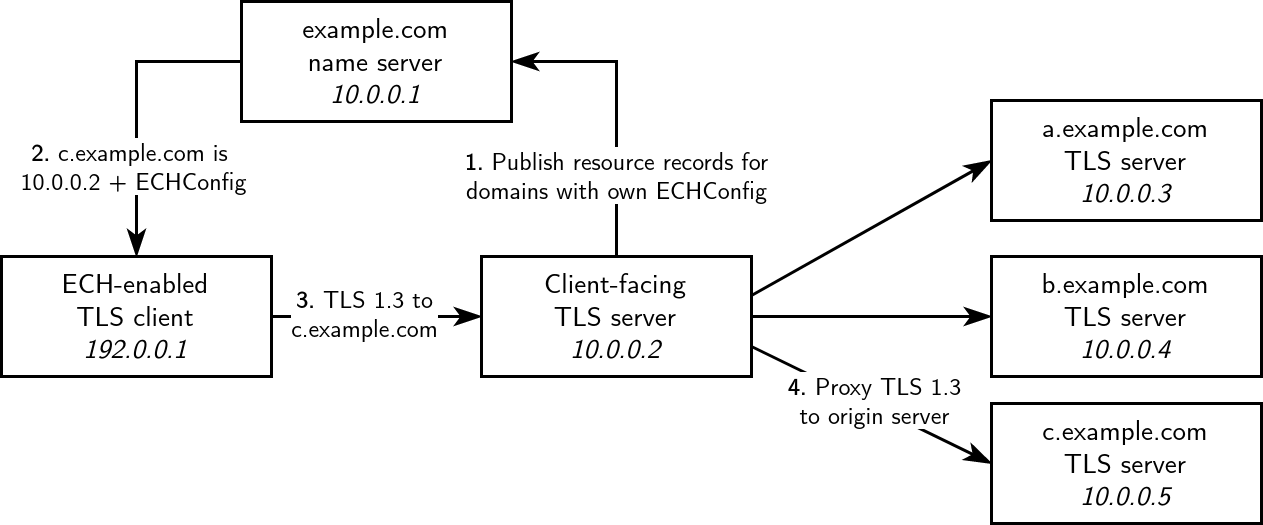
\includegraphics[width=160mm]{images/ech-split-mode.png}}
\caption[Example execution of ECH in Split Mode]{An example of how ECH can be used in Split Mode when the ECH-service provider is not co-located with the requested private domain origin server. Steps 1 and 2 are completed out-of-band. Steps 3 and 4 result in a TLS connection being established between the client and origin server.}
\label{ech_split_mode_figure}
\end{figure}

Split Mode is crucial for unbinding the provider from the origin server which is necessary for being able to handle more diverse ECH deployment scenarios. This is generally required when the provider does not have the resources to complete the TLS connection and must proxy the connection to the requested origin server. This can be the case in cloud hosting environments, where the private keys and certificates of hosted services belong to the customer and cannot be accessed by the reverse proxies operated in front of the internal cloud network infrastructure. However, if the client, provider and origin server are separated by a public network such that traffic on both the client to provider and provider to origin server channels can be intercepted by a foreign network observer, it is not enough to encrypt this traffic with TLS 1.3 to prevent the observer from learning which origin server the client is interacting with, which may eliminate any privacy offered to the client by the provider's anonymity set. This is possible through an attack accomplished using traffic analysis.







\section{Traffic Analysis}

Traffic analysis is the process of passively recording and inspecting possibly large amounts of messages sent over a network in order to discern information not apparent when considering each message in isolation. Traffic analysis techniques can be used to infer sensitive information from patterns in network activity regardless of channel encryption as they exploit fundamental aspects inherent to how a communication system is implemented. For example, consider that the mere presence of network traffic between a household and a specific medical, educational or political institution's web server might tell us a great deal about the lifestyle and affiliations of the occupants without needing to know anything about the contents of the traffic itself. Aside from analysing traffic behaviour, other techniques include inspecting network protocols being used, observing changes in round-trip latency and comparing packet sizes and contents.

\subsection{Traffic Correlation Attacks}

Traffic correlation attacks describe a large subset of traffic analysis techniques identified by their use of correlating patterns found in network channels to detect associations between entities that were otherwise not evident. These can typically be used to unmask users and their activities in anonymisation networks. Back, Möller, and Stiglic have reported on correlation metrics such as packet counting and traffic shaping employed against the Freedom network while DeFabbia-Kane has additionally found packet timing and inter-packet delay to be effective against Tor~\cite{back2001traffic, defabbia2011analyzing}. Most significantly for this paper, Trevisan et al. have shown ECH operating over a public network is highly susceptible to traffic correlation attacks using a conventional machine learning algorithm trained on information extracted from the IP, TCP and UDP protocol fields, TLS SNI values, packet sizes and inter-packet delays~\cite{trevisan2023attacking}.

\subsection{Countermeasures}

The effectiveness of traffic correlation attacks can be mitigated by disrupting the recognisable patterns in communication through removing distinctive features and inserting randomness into messages and traffic flow. Back, Möller, and Stiglic saw how PipeNet introduces dummy packets into the network between correspondents as traffic padding and uses mixing and pacing with a packet scheduling algorithm at each node to hinder attack vectors.

This is a particularly hard challenge for low-latency network systems such as web servers and instant-messaging platforms because many mitigations require the introduction of unacceptable delays or continuous high bandwidth usage. Levine et al. conducted a study on using packet timing analysis to attack low-latency anonymisation networks and concluded the effectiveness of traffic padding can be improved by intentionally occasionally dropping dummy packets~\cite{levine2004timing}. Wright, Coull and Monrose have suggested morphing classes of encrypted traffic into indistinguishable distributions with a mathematical model for minimising differing features over time~\cite{wright2009traffic}.









\section{Summary}

TLS and DNS continue to evolve as their requirements shift in response to modern security and privacy demands. From this movement, the ECH extension for TLS 1.3 has emerged to enable the encryption of the ClientHello message and thereby addressing one of the last points an attacker can learn of potentially sensitive information such as the SNI and ALPN list. The ECH standard defines Split Mode as a network topology which permits the ECH-service provider to be physically separate from the origin server. However, such a situation reveals a potential attack surface against the extension through traffic correlation, which must be disrupted using various practical countermeasures.

\chapter{Design}\label{Design}

<this disseration aims to serve as a guide for security researchers and service operator on the viablity of distributed ech>
<during the course of this project, a system design was formulated and iteratively refined>
<the main parts of the design considered are its deployment schema and protecting traffic>

<in this chapter, we will study the determined solution as well as the challenges that motivated its design>
<this consists of a overview of purposed system followed by an examination of its individual components>



\section{Problem Overview}

<ech split mode serves as a bases for distributed deployment, but makes no attempt to address the implications of servers being operated by separate organisations and located across a public network>
<to do so, we must consider a number of challenges faced by this situation to enable co-operation and secure functioning>
<this paper purposes a loose network of tls servers all acting as ech providers for each other which proxy connections to the true origin server, as depicted in Fig.~\ref{distributed_ech_figure}>

\begin{figure}[ht]
\centerline{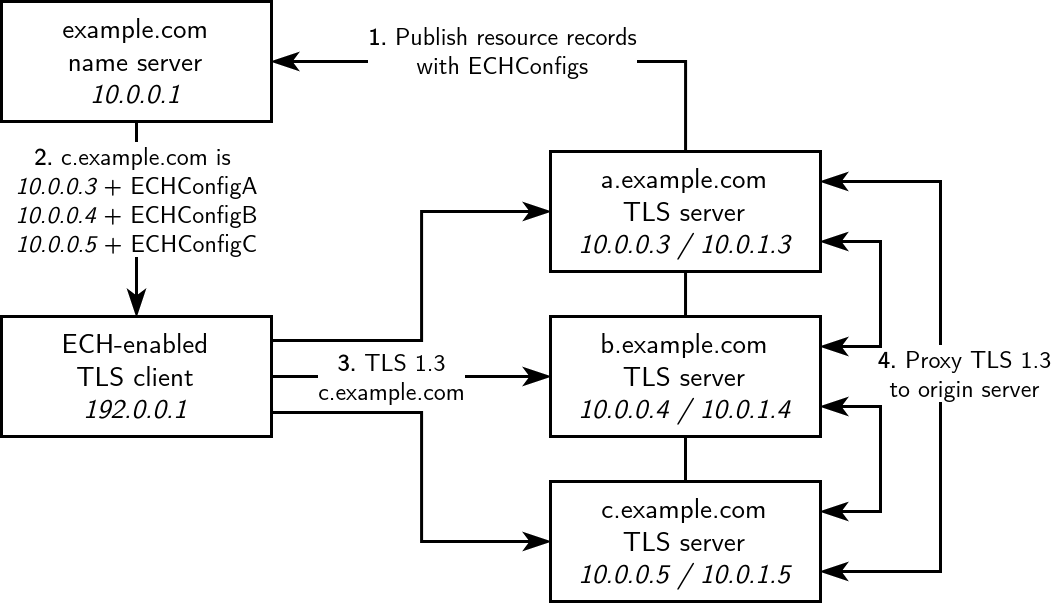
\includegraphics[width=160mm]{images/distributed-ech.png}}
\caption[Example distributed ECH deployment]{<>}
\label{distributed_ech_figure}
\end{figure}

<parallel to the operation of ech split mode>
<loose network must publish appropriate resource records such that clients choose to query any of them for any of their domains>
<all providers listens on their public facing network interface for with ClientHelloOuter>
<providers also listens on a virtual private network interface they are all a part of for actual connections>
<clients resolve requested domain using DoH and then use round robin or other selection process to uniformly choose one of the providers at random with the correct echconfig>
<client begins establishment to the requested via the selected provider using the providers echconfig>
<as in ech split mode, the provider decrypts the ClientHelloInner to retrieve the actual domain requested>
<the provider maps the domain to the true origin server and proxies the clients connection over a backend communication network to the origin server>
<the origin server listening on the vpn interface completes the tls handshake with the client through the provider>
<this connection is end-to-end encrypted, so the provider does not mitm>

<the design challenges can be split into two topics, mechanism for distribution and traffic obfuscation>
<the distribution mechanism deals with a couple designs for the a dns publication schema so compatible clients follow the above process, and the networking required for tls servers to communicate with each other>
<this considers load distribution, echconfig and stream proxying over a virtual private network>







\section{Distribution Mechanism}

<distribution is based on two parts>
<first, clients need to be able to select from several options provided by a dns query>
<second, co-oerating tcp servers need to be able to forward connections to each other based on the decrypted ClientHelloInner>

\subsection{DNS Publication Schema}

<one approach: shared echconfig with round robin A resource records>
<load is evenly distributed across servers because client uses round robin on selected A rrs>
<but requires shared secrets between all servers as there is no way to specify which ech key is associated with which host>
<another approach: using alternative endpoints to associate ech keys with individual servers>
<load is evenly distributed across servers due to matching priority>
<unfortunately more fine-grained load distribution is not possible without srv resource records adoption>
<we can replicate this using a dynamic dns service, where records are regularly substituted such that load is distributed across servers in a fair manner>

\subsection{TLS Server Co-operation}

<tls servers are physically separate from each other and must communicate over the same network as the client when forwarding the client connection>
<to do this, a virtual private network is established between participating servers>
<servers still listen for normal tls connections on 443 port of the public interface as well as ech-enabled connection>
<ech split mode connections have their ClientHelloInner decrypted and private domain mapped to the actual origin>
<clients connection is forwarded over a virtual private network to the origin server>
<the origin server listening on the vpn interface completes the tls handshake with the client through the provider>







\section{Traffic Obfuscation}

<ech is susceptible>\cite{trevisan2023attacking}
<correlation attacks in low-latency systems like web browsing and video streaming compared to high-latency like email>\cite{levine2004timing}
<rx/tx timing> <packet lengths> <traffic patterns> \cite{defabbia2011analyzing}

\begin{figure}[ht]
\centerline{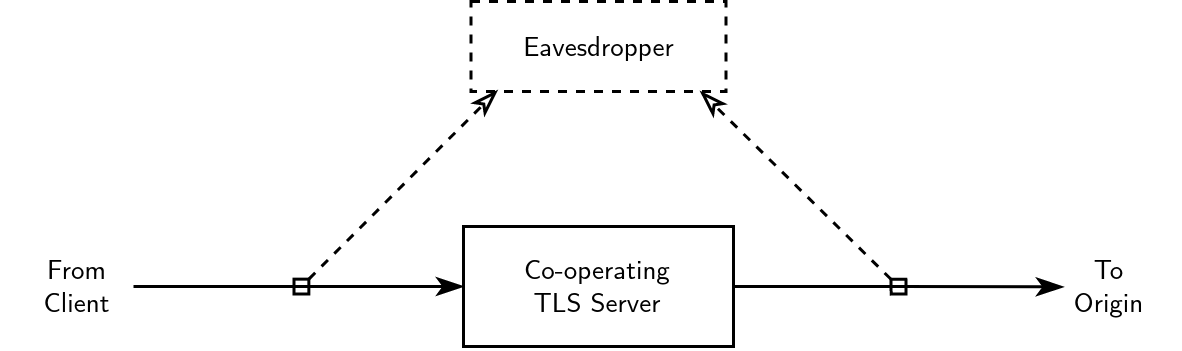
\includegraphics[width=150mm]{images/correlation-attack.png}}
\caption[Diagram of various traffic metrics useful in correlation attacks]{<TODO>}
\label{correlation_figure}
\end{figure}

<traffic obfuscation techniques lead "to disrupt the patterns">

\subsection{Normalisation}

<shannon and perfect secrecy: removal of all identifying features>
<injection of dummy traffic to fill bandwidth gaps>
<impracticality in civilian environments due to required bandwidth>

\subsection{Pacing and Mixing}

<while not perfect, many practical techniques exist to mask traffic with minimal impacts>
<padding packets themselves to prevent packet length correlation>
\cite{yu2012predicted}
<to disrupt timing-based correlation attacks, delays and slotting (aka pacing) can be used>
<to disrupt deep packet inspection, other packet-based correlation attacks (traffic patterns), traffic mixing can be used>
\cite{fu2003analytical, fu2003effectiveness}
<a simple technique is packet duplication, where a similar packet is sent to every peer>

% TODO: likely a comparison table or graph from info theory
% \begin{figure}[ht]
% \centerline{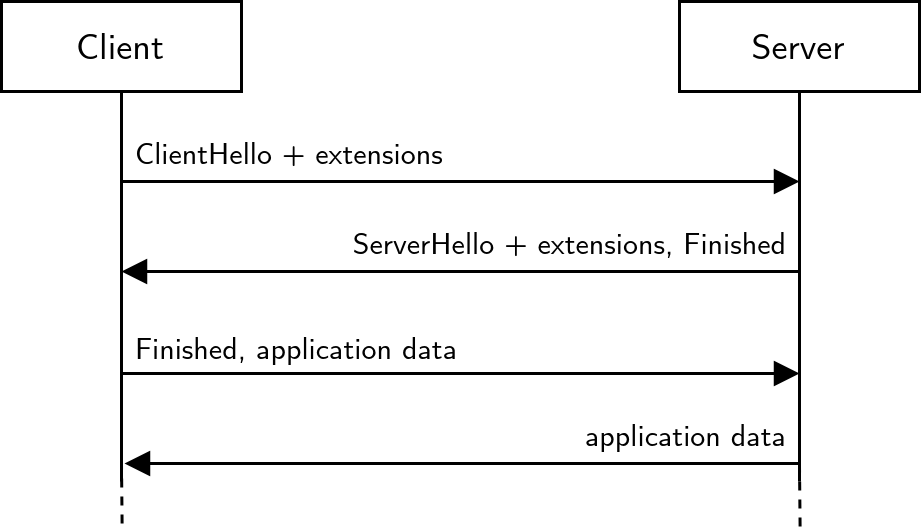
\includegraphics[width=120mm]{images/tls-handshake.png}}
% \caption[TODO technique comparision]{<TODO>}
% \label{noise_figure}
% \end{figure}





\section{Summary}

<it fulfills the desired design criteria>
<we use dns https rrs to distributed load across multiple ech providers>
<separate echconfigs can be used be each server as the ech key is associated with the server>
<an alternative strategy exists that is more robust but requires shared echconfig>
<a virtual private network between co-operating servers is used to allow peer communication>
<ech split mode is vulnerable to correlation attacks>
<but techniques exist to defend against attacks>

\chapter{Implementation}\label{Implementation}

\blindtext









\section{Simulation}

\blindtext

\subsection{Virtualisation}

qemu+debvm
\blindtext

\begin{listing}[ht]
\inputminted{bash}{snippets/build.bash}
\caption[Building OpenSSL from source inside build.img with DebVM]{TODO builder}
\end{listing}

\subsection{Networking}

\blindtext

\begin{listing}[ht]
\inputminted{bash}{snippets/br0.bash}
\caption[Connecting QEMU virtual machines using a network bridge]{TODO br0}
\end{listing}

\blindtext

\begin{listing}[ht]
\inputminted{ini}{snippets/br0.ini}
\caption[Static bridge network configuration using systemd]{TODO /etc/systemd/network/00-br0.network contents}
\end{listing}

\blindtext

\begin{listing}[ht]
\inputminted{bash}{snippets/root.bash}
\caption[Generating a new self-signed root CA X.509 certificate using OpenSSL]{TODO root ca}
\end{listing}

\blindtext










\section{DNS Server}

\blindtext

\begin{listing}[ht]
\inputminted{bash}{snippets/dns.bash}
\caption[Signing a new X.509 certificate for ns.example.com using OpenSSL]{TODO dns}
\end{listing}

\blindtext

\begin{listing}[ht]
\inputminted{bash}{snippets/bind}
\caption[DNS over HTTPS configuration using BIND 9]{TODO /etc/bind/named.conf contents}
\end{listing}

\blindtext

\begin{listing}[ht]
\inputminted{zone}{snippets/example.zone}
\caption[Zone file for example.com zone with distributed ECH]{}
\end{listing}

\blindtext











\section{TLS Server}

\blindtext

\subsection{Peer Communication}

\blindtext

\begin{listing}[ht]
\inputminted{bash}{snippets/host_wg.bash}
\caption[Generating a new WireGuard key pair for tcd.example.com]{TODO host wg}
\end{listing}

\blindtext

\begin{listing}[ht]
\inputminted{ini}{snippets/host_wg.ini}
\caption[Configuring a WireGuard network interface using systemd]{TODO host wg}
\end{listing}

\begin{listing}[ht]
\inputminted{ini}{snippets/host_wg0.ini}
\caption[Static WireGuard network configuration using systemd]{TODO host wg0}
\end{listing}

\blindtext

\subsection{Web Server}

\blindtext

\begin{listing}[ht]
\inputminted{bash}{snippets/host_tls.bash}
\caption[Generating a new ECH key pair for tcd.example.com using OpenSSL]{TODO host+site tls}
\end{listing}

\blindtext

\begin{listing}[ht]
\inputminted{nginx}{snippets/nginx}
\caption[Distributed ECH NGINX configuration for tcd.example.com]{TODO nginx}
\end{listing}

\blindtext

\begin{listing}[ht]
\inputminted{bash}{snippets/padding.bash}
\caption[Rudimentary script to shroud legitimate WireGuard communication]{}
\end{listing}

\blindtext











\section{TLS Client}

\blindtext


\subsection{curl}

\blindtext

\begin{listing}[ht]
\inputminted{nginx}{snippets/curl.bash}
\caption[Command to use ECH-enabled curl on QEMU virtual machines]{TODO curl}
\end{listing}

\blindtext

\begin{figure}[ht]
\centerline{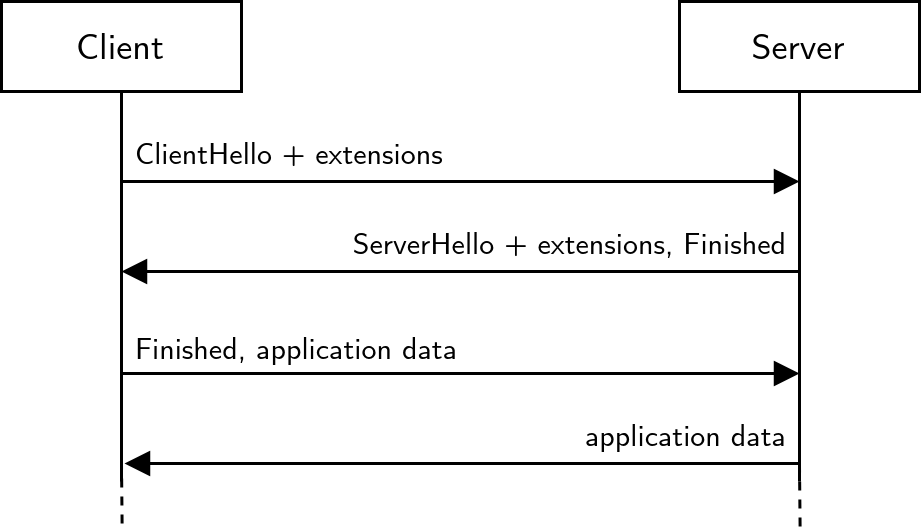
\includegraphics[width=120mm]{images/tls-handshake.png}}
\caption[Screenshot of curl output when accessing tcd.example.com]{<TODO>}
\label{curl_screenshot_figure}
\end{figure}

\subsection{Mozilla Firefox}

\blindtext

\begin{figure}[ht]
\centerline{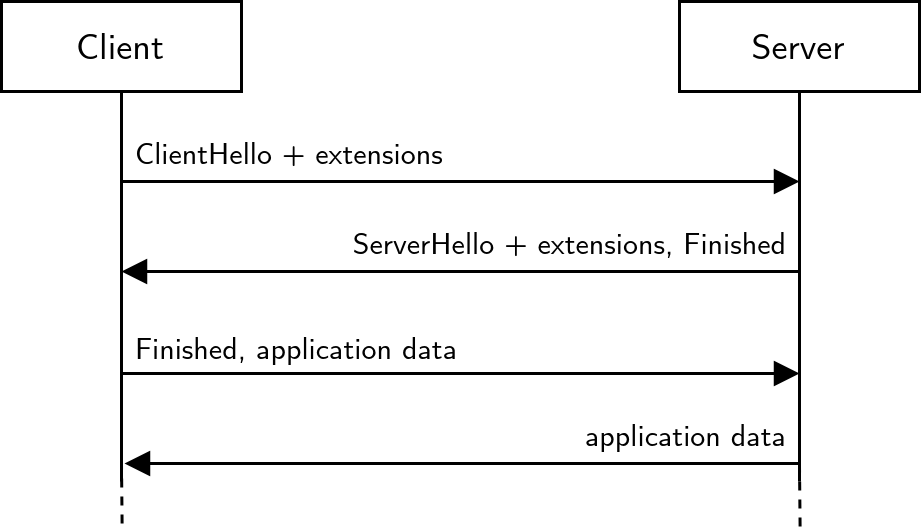
\includegraphics[width=120mm]{images/tls-handshake.png}}
\caption[Screenshot of Mozilla Firefox when accessing tcd.example.com]{<TODO>}
\label{firefox_screenshot_figure}
\end{figure}

\subsection{Google Chrome}

\blindtext

\begin{figure}[ht]
\centerline{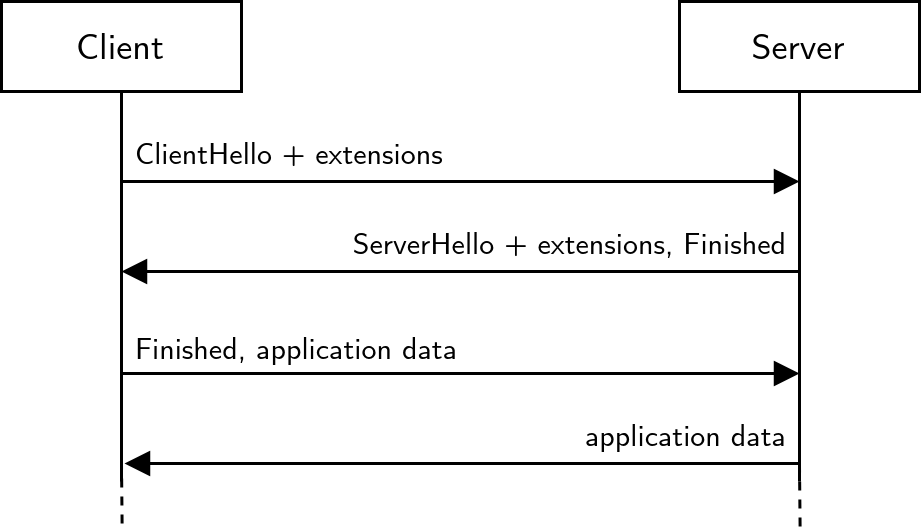
\includegraphics[width=120mm]{images/tls-handshake.png}}
\caption[Screenshot of Google Chrome when accessing tcd.example.com]{<TODO>}
\label{chrome_screenshot_figure}
\end{figure}











\section{Summary}

\blindtext

\chapter{Results and Discussion}\label{Results}

\blindtext









\section{Data Collection}

\blindtext









\section{Evaluation}

\blindtext

\subsection{Performance}

\blindtext

\subsection{Security}

\blindtext









\section{Limitations}

\blindtext

\subsection{Load Balancing}

\blindtext

\subsection{Traffic Padding}

\blindtext









\section{Summary}

\blindtext

\chapter{Conclusion}\label{Conclusion}

<this research has been a first effort to create a distributed ech deployment model>
<we have seen background>
<we have seen design>
<we have seen implementation>
<we have seen results>

<in this final chapter, present key learnings>
<then outline future work>
<finish with a reflection of the project as a whole>









\section{Learnings}

<ECH Split Mode topology permits distributed deployment>
<https rr enable static load distribution>
<A dynamic DNS service allows for fair load distribution>
<minimal performance impact when compared to normal>
<security is ok and techniques exist to defend against correlation attacks>









\section{Future Work}

<shared dns publication strategy (with ech key rotation)>
<dynamic traffic flow analysis for load balancing (instead of just distribution)>
<more in-depth study on disrupting traffic correlation attacks>
<test deployment on actual hardware with realistic traffic>








\section{Reflection}

<what i think went well>
<reliable, reproducable and deterministic virtual environment test bed>
<functioning distributed ech prototype>
<if i was to do this again, what would i change>
<dedicate more time to theoretical instead of practical (e.g. got firefox working but unsure if actually compatible with spec>
<however, the work completed is still applicable to future effort>

\printbibliography
\addcontentsline{toc}{chapter}{Bibliography}

\appendix
\renewcommand{\thechapter}{A\arabic{chapter}}
\chapter{Project Files}\label{project-files}

For the sake of experimental reproducibility, a ZIP archive of the project code, three scenarios and packet capture files have been provided alongside this report. Additionally, a copy can be found online: \url{https://github.com/tedski999/distributed-ech}.

The source code consists of a single Bash script, \mintinline[linenos=false,fontsize=]{bash}{run.sh}, which contains all the necessary logic to setup and run any virtual testing environment described using two scenario configuration files, \mintinline[linenos=false,fontsize=]{bash}{network.csv} and \mintinline[linenos=false,fontsize=]{bash}{server.csv}. The script is dependent on DebVM, and by extension QEMU and mmdebstrap. A path \mintinline[linenos=false,fontsize=]{bash}{sandbox} must also be specified as the directory to store QEMU images and other ephemeral data.

Given two scenario configuration files, the environment can be generated and started by executing \mintinline[linenos=false,fontsize=]{bash}{./run.sh sandbox network.csv servers.csv}. Initial setup times can be lengthy, as OpenSSL, curl and NGINX must be built before all QEMU virtual machine images are configured and booted. These builds and configurations are preserved, so later environment boot up times are far quicker.

Once running, a virtual machine can be accessed using the corresponding SSH command printed to the terminal: \mintinline[linenos=false,fontsize=]{bash}{ssh -i 'sandbox/ssh.key' -p 2222 root@127.0.0.1}. See Chapter~\ref{Implementation} for more information on how to use this environment.

\chapter{Verbose curl Output}\label{verbose-curl-output}

\inputminted[tabsize=2,breaklines,breakanywhere]{text}{snippets/curl}


\end{document}
